\documentclass[titlepage,a4paper]{article}

\usepackage{a4wide}
\usepackage[colorlinks=true,linkcolor=black,urlcolor=blue,bookmarksopen=true]{hyperref}
\usepackage{bookmark}
\usepackage{fancyhdr}
\usepackage[spanish]{babel}
\usepackage[utf8]{inputenc}
\usepackage[T1]{fontenc}
\usepackage{graphicx}
\usepackage{float}

\graphicspath{ {imagenes/} }  % Las imagenes las reubique en la carpeta imagenes

\pagestyle{fancy} % Encabezado y pie de página
\fancyhf{}
\fancyhead[L]{TP1}
\fancyhead[R]{Algoritmos y Programación III - FIUBA}
\renewcommand{\headrulewidth}{0.4pt}
\fancyfoot[C]{\thepage}
\renewcommand{\footrulewidth}{0.4pt}

\begin{document}
\begin{titlepage} % Carátula
	\hfill
\includegraphics[width=6cm]{logofiuba.jpg}
    \centering
    \vfill
    \Huge \textbf{Trabajo Práctico 1 — Smalltalk}
    \vskip2cm
    \Large [7507/9502] Algoritmos y Programación III\\
    Curso 2 \\ % Curso 1 para el de la tarde y 2 para el de la noche
    Primer cuatrimestre de 2020 
    \vfill
    \begin{tabular}{ | l | l | } % Datos del alumno
      \hline
      Alumno: & Paredes Ramirez, Luis Jose \\ \hline
      Número de padrón: & 104851 \\ \hline
      Email: & lparedesr@fi.uba.ar \\ \hline
  	\end{tabular}
    \vfill
    \vfill
\end{titlepage}

\tableofcontents % Índice general
\newpage

\section{Introducción}\label{sec:intro}
  El presente informe reune la documentacion del primer trabajo practico de la materia
  Algoritmos y Programación III que consiste en desarrollar un sistema que permita encontrar el mejor 
  presupuesto de un pintor de acuerdo a las necesidades de los clientes. \newline

  Este trabajo es desarrollado usando los conceptos del paradigma de la orientación a objetos
  utilizando el sistema Smalltalk.


% Deberá contener explicaciones de cada uno de los supuestos que el alumno haya tenido que adoptar a partir de 
% situaciones que no estén contempladas en la especificación.
\section{Supuestos}\label{sec:supuestos}

Los siguientes supuestos se tomaron como constantes que siempre se cumpliran en el trabajo practico.

  \subsection{Pincel}
    \begin{itemize}
      \item El pintor que utiliza Pincel siempre tarda 2 horas en pintar un $M^2$
      \item El pintor que utiliza Pincel siempre gastara 4 litros por $M^2$
      \item El pintor que utiliza Pincel dara un descuento del 50\% para proyectos mayores a 40 $M^2$
    \end{itemize}

  \subsection{Rodillo}
    \begin{itemize}
      \item El pintor que utiliza Rodillo siempre tarda 1 horas en pintar un $M^2$
      \item El pintor que utiliza Rodillo siempre gastara 5 litros por $M^2$
      \item El pintor que utiliza Rodillo no aplica descuento para proyectos mayores a 40 $M^2$
    \end{itemize}

  \subsection{Alba}
    \begin{itemize}
      \item Pintura Alba siempre requiere 1 mano con pincel o 1 mano con rodillo
    \end{itemize}

  \subsection{Venier}
    \begin{itemize}
      \item Pintura Venier siempre requiere 2 manos con pincel o 1 mano con rodillo
    \end{itemize}
  

% Uno o varios diagramas de clases mostrando las relaciones estáticas entre las clases. 
% Puede agregarse todo el texto necesario para aclarar y explicar su diseño. 
%Recuerden que la idea de todo el documento es que quede documentado y entendible cómo está implementada la solución.
\newpage
\section{Diagramas de clase}\label{sec:diagramasdeclase}
Uno o varios diagramas de clases mostrando las relaciones estáticas entre las clases.  
Puede agregarse todo el texto necesario para aclarar y explicar su diseño. 
Recuerden que la idea de todo el documento es que quede documentado y entendible cómo está implementada la solución. 
Todos los diagramas tienen que estar embebidos como imágenes en el informe de manera tal que entren en el ancho de una hoja A4 
sin tener que rotarla.  No se aceptarán diagramas en archivos sueltos. 


% \footnote{Mensaje debajo}
%%%%%%%%%%%%%%%%%%%%%%%%%%%%%%%%%%%%%%%%%%%%%%%%%%%%%%%%%%% Cambiar  %%%%%%%%%%%%%%%%%%%%%%%%%%%%%%%%%%%%%%%%%%%%%%

\begin{figure}[H]
  \centering
  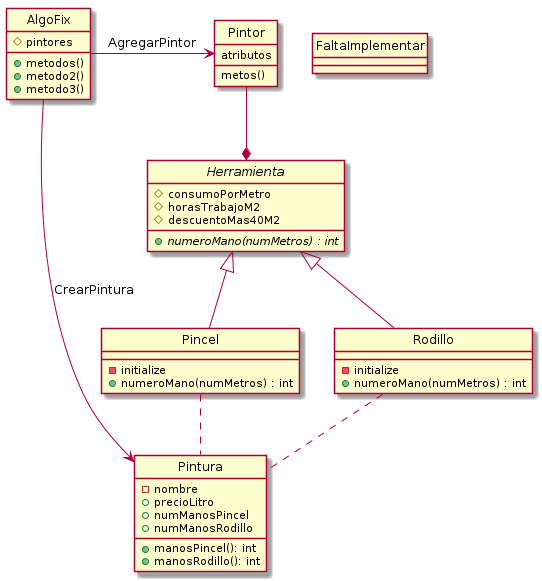
\includegraphics[width=0.8\textwidth]{diagrama_clase01.png}
  \caption{\label{fig:class01}Prueba Diagrama de Clase.}
  \end{figure}

%%%%%%%%%%%%%%%%%%%%%%%%%%%%%%%%%%%%%%%%%%%%%%%%%%%%%%%%%%% Cambiar  %%%%%%%%%%%%%%%%%%%%%%%%%%%%%%%%%%%%%%%%%%%%%%

\begin{figure}[H]
\centering
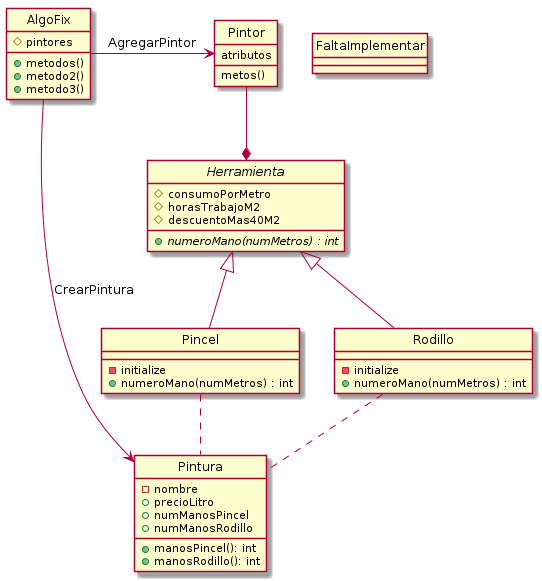
\includegraphics[width=0.8\textwidth]{diagrama_clase01.png}
\caption{\label{fig:class02}Diagrama de Clase 2.}
\end{figure}

%%%%%%%%%%%%%%%%%%%%%%%%%%%%%%%%%%%%%%%%%%%%%%%%%%%%%%%%%%% Cambiar  %%%%%%%%%%%%%%%%%%%%%%%%%%%%%%%%%%%%%%%%%%%%%%


% Explicaciones sobre la implementación interna de algunas clases que consideren que puedan llegar a resultar interesantes.
\section{Detalles de implementación}\label{sec:implementacion}
\begin{itemize}
  \item Por decisión de diseño las excepciones intentarán salir al no mas crear los objetos. Es decir, si en la creacion de un Pincel o Pintura se
  le pasa algun valor invalido lanzará la excepcion \textbf{ValorInvalido} en el momento de su creación. Sin embargo, adicionalmente para darle mayor robustez al programa, en los casos bordes donde por alguna razon
  llega algun valor invalido a las operaciones esperadas, lanzara la excepcion \textbf{ValorInvalido} y asi evitar resultados absurdos.
  \item Se tomaran los supuestos hechos en la sección \textbf{\ref{sec:supuestos}} como invariantes en todo momento del programa,
  por tanto las propiedades propias de cada objeto se asignan en su inicializacion en el momento de su creacion.
\end{itemize}


\subsection{Nota de los tests}
De las pruebas integradoras se extrajeron cada una de las pruebas unitarias de 
\newline AlgoFixTestUnitarios de modo de simplificar el panorama y enfocar 
unicamente la atencion en resolver un problema a la vez. 
De este modo su proposito es cumplir con las pruebas por separado para que luego 
pasen las pruebas integradoras. \newline

Adicionalmente se creo una clase de prueba por cada clase que se creó para resolver el trabajo practico
en las cuales se pone a prueba el comportamiento esperado del objeto en tiempo de ejecucion. Por tanto
las pruebas de AlgoFix estan orientadas a que el objeto AlgoFix se comporte como es de esperar en tiempo de ejecucion, 
y es distinto de las otras pruebas.


% Explicación de cada una de las excepciones creadas y con qué fin fueron creadas.
\section{Excepciones}\label{sec:excepciones}
\begin{description}
\item[Exception \underline{ValorInvalido:}] Excepcion lanzada en caso de pasarle un parametro que no haga sentido para el comportamiento esperado del objeto.

Se usa al pasarle un \textbf{numMetros} invalido al Pintor o a la Herramienta, y tambien cuando se pasa un \textbf{numLitros} invalido a la Pintura.
\end{description}


% Mostrar las secuencias interesantes que hayan implementado. Pueden agregar texto para explicar si algo no queda claro.
\section{Diagramas de secuencia}\label{sec:diagramasdesecuencia}
Mostrar las secuencias interesantes que hayan implementado. Pueden agregar texto para explicar si algo no queda claro. 

%%%%%%%%%%%%%%%%%%%%%%%%%%%%%%%%%%%%%%%%%%%%%%%%%%%%%%%%%%% Cambiar  %%%%%%%%%%%%%%%%%%%%%%%%%%%%%%%%%%%%%%%%%%%%%%
\begin{figure}[H]
\centering
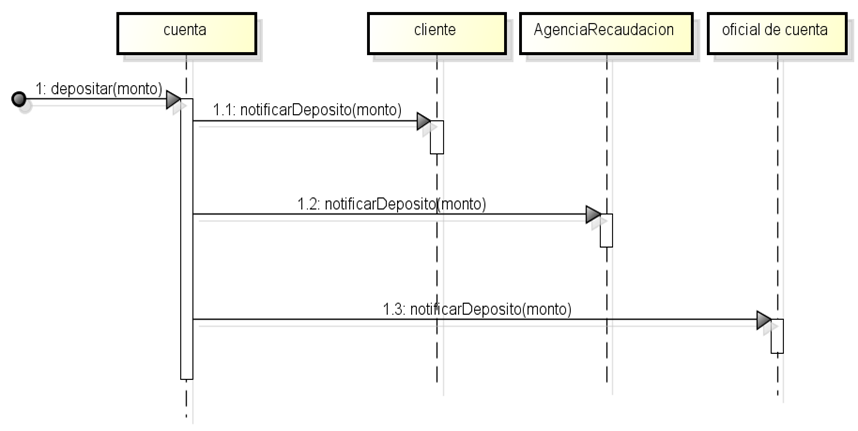
\includegraphics[width=0.8\textwidth]{diagrama_secuencia01.png}   %CAMBIAR ACA EL DIAGRAMA
\caption{\label{fig:seq01}Comportamiento esperado de depositar.}
\end{figure}

Implementar

\begin{figure}[H]
\centering
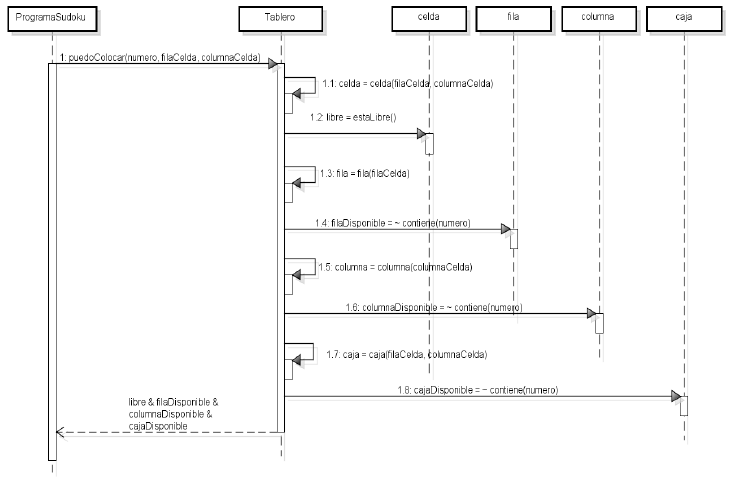
\includegraphics[width=\textwidth]{diagrama_secuencia02.png}
\caption{\label{fig:seq02}Diagrama de Secuencia de puedoColocar().}
\end{figure}

Implementar

\end{document}